%!TEX root = ../thesis.tex
\chapter{Transformation Implementation}
\label{ch:trans-implementation}

% TODO find a better word than 'guidelines'

\section{Guidelines}

In general, when designing the \yauhau{} graph transformation, I have opted for a simplicity focused approach.
The following sections describe some properties of the algorithms which I have tried to adhere to as much as possible.

\subsection{Single Concern}

Each transformation should be as self contained as possible.
The less overlap there is between any two graph transformations the easier they are to implement and the easier to debug.

Therefore both context rewrites \texttt{if} and \texttt{smap} are separate transformations which are combined using the generalised context rewrite algorithm.
None of those rewrites know of the other.
If and smap have no overlap in the types of nodes they insert or delete (apart from the \fetch{} node of course for which both of them change the associated context stack).
Also the combining context rewrite has no knowledge of the inner workings of any of the individual unwinding transformations.
Its only concern is to correctly handle nesting.
Therefore it simply dispatches rewrites based on type of context encountered.
Rewrites are basically just implementations of an interface.

\subsection{No complicated edge case optimisation}

No regards for special cases unless necessary for semantic correctness.
Algorithms should handle the problem as generic as possible.
This makes the implementation simpler, as less special cases have to be distinguished.
The generic implementation of course is required to be semantic preserving for all cases, which often means inserting redundant operators.

In general this rule introduces a fair number of redundant operators.
The worst perpetrator of this is an operator called \texttt{identity} which is used to preserve destructuring in fetches on if branches.
When two fetches which were on different branches of the same if are merged together it may be that one of the fetches had its return be destructured differently than the other.
If this is the case the (IR) returns of those ifs cannot be unified.
Therefore a new binding is added leading from the combined fetch to two \texttt{identity} operators.
Each of the \texttt{identity} operators is destructured like one of the former two fetches and wired to the same subsequent nodes respectively.
A context arc from the \texttt{ifThenElse} operator selects one of the \texttt{identity} operators at runtime depending of the active branch.

The reason this is so inefficient is that, other than destructuring data, the \texttt{identity} operator does literally nothing, thus we have to schedule a bunch of operators at runtime which are essentially NoOp's.

\section{Separate Optimisations}

To get back the lost efficiency from the naive and simple transformations \yauhau{} separately introduces an optimisation pass.
This means the overall transformation is divided into three steps

\begin{enumerate}
    \item \textbf{Context unwinding.} Rewriting all contexts around fetches such that every fetch is only called once.
    \item \textbf{Batching.} Replacing all fetches with rounds of accumulated fetches.
    \item \textbf{Optimisations.} Clean up the graph, remove redundant operators.
\end{enumerate}

Optimisations of this kind are very high level.
They operate entirely on the dataflow IR and only concern themselves with \yauhau{} and Ohua internal operators.
Optimisations are repeated until the graph does not change anymore.


\subsection{Identities}

As a result of, in particular the if rewrite, a lot of \texttt{identity} operators get added to the graph and not all of them are strictly necessary.
The typical use of an \texttt{identity} operator is to destructure a piece of data, see Figure~\ref{fig:identity-example}.
This is used after the if rewrite to destructure the data differently  depending on the chosen branch.
Since the identity operator itself doesn't actually perform any calculation flow of the form seen in Figure~\ref{fig:redundant-identity-example} has no practical use.
This optimisation removes those kinds of identities.
Specifically if the output of an identity operator is not destructured then there is no need for it, hence it can be removed and each occurrence of the return binding is replaced by the input binding and a potential context arc is connected to the recipient as well, see Figure~\ref{fig:redundant-identity-example-rewritten}.

\begin{figure}
    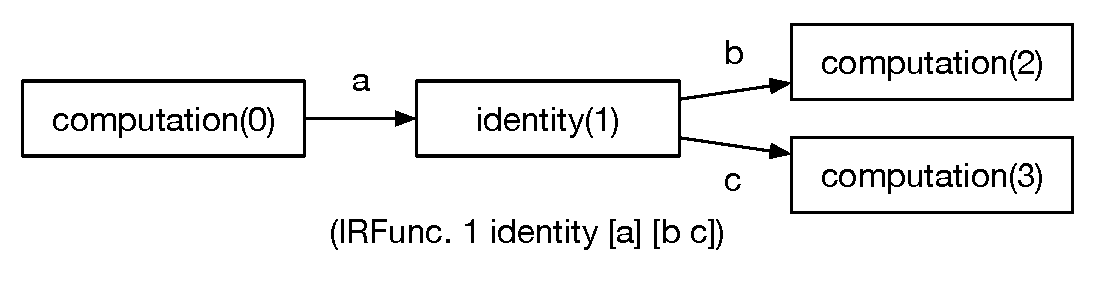
\includegraphics[width=\linewidth]{../Figures/identity-example}
    \caption{Identity use example}
    \label{fig:identity-example}
\end{figure}

\begin{figure}
    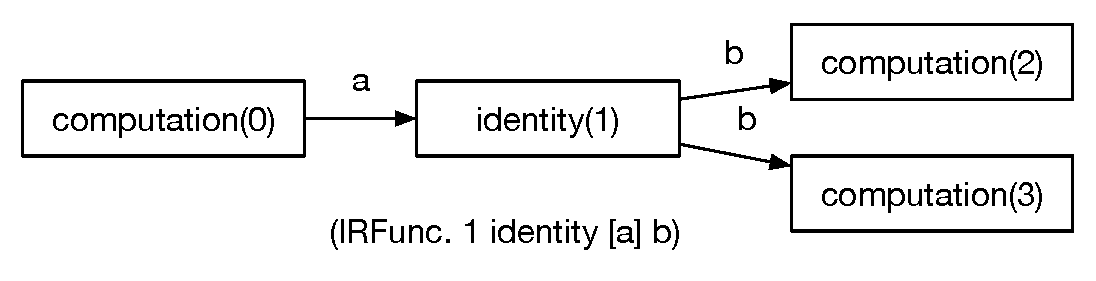
\includegraphics[width=\linewidth]{../Figures/redundant-identity-example}
    \caption{Redundant identity example}
    \label{fig:redundant-identity-example}
\end{figure}

\begin{figure}
    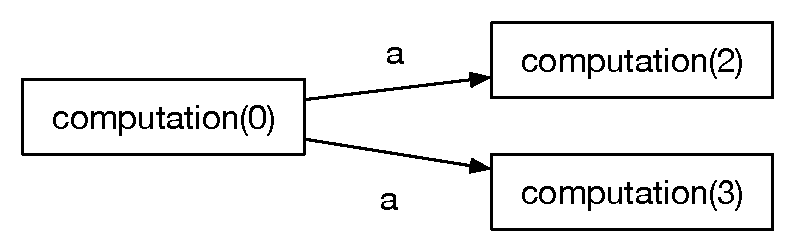
\includegraphics[width=\linewidth]{../Figures/redundant-identity-example-rewritten}
    \caption{Optimised flow}
    \label{fig:redundant-identity-example-rewritten}
\end{figure}

A second \texttt{identity} optimisation is the removal of duplicate identities.
If two identities with the same input are destructured into the same output they are redundant.
Both are removed from the graph and data is destructured at the source.
Both context arcs are connected to the respective recipients.
